
\documentclass[12pt]{article}

% Layout.
\usepackage[top=1in, bottom=0.75in, left=1in, right=1in, headheight=1in, headsep=6pt]{geometry}

% Fonts.
\usepackage{mathptmx}
\usepackage[scaled=0.86]{helvet}
\renewcommand{\emph}[1]{\textsf{\textbf{#1}}}

% TiKZ.
\usepackage{tikz, pgfplots,mathrsfs}
\usetikzlibrary{calc}
\pgfplotsset{compat = newest}
 
\pgfplotsset{my style/.append style={axis x line=middle, axis y line=
middle, xlabel={$x$}, ylabel={$y$}, axis equal
}}

% Misc packages.
\usepackage{amsmath,amssymb,latexsym}
\usepackage{graphicx}
\usepackage{array}
\usepackage{xcolor}
\usepackage{multicol}

% Commands to set various header/footer components.
\makeatletter
\def\doctitle#1{\gdef\@doctitle{#1}}
\doctitle{Use {\tt\textbackslash doctitle\{MY LABEL\}}.}
\def\docdate#1{\gdef\@docdate{#1}}
\docdate{Use {\tt\textbackslash docdate\{MY DATE\}}.}
\def\doccourse#1{\gdef\@doccourse{#1}}
\let\@doccourse\@empty
\def\docscoring#1{\gdef\@docscoring{#1}}
\let\@docscoring\@empty
\def\docversion#1{\gdef\@docversion{#1}}
\let\@docversion\@empty
\makeatother

% Headers and footers layout.
\makeatletter
\usepackage{fancyhdr}
\pagestyle{fancy}
\fancyhf{} % Clears all headers/footers.
\lhead{\baselineskip 30pt
%\emph{\@doctitle\hfill\@docdate}
\emph{\@docdate\hfill\@doctitle}
\ifnum \value{page} > 1\relax\else\\
\emph{Name: \rule{3.5in}{1pt}\hfill \@docscoring}\fi}
\rfoot{\emph{\@docversion}}
\lfoot{\emph{\@doccourse}}
\cfoot{\emph{\thepage}}
\renewcommand{\headrulewidth}{0pt}%
\makeatother

% Paragraph spacing
\parindent 0pt
\parskip 6pt plus 1pt

% A problem is a section-like command. Use \problem{5} to
% start a problem worth 5 points.
\newcounter{probcount}
\newcounter{subprobcount}
\setcounter{probcount}{0}
\newcommand{\problem}[1]{%
\par
\addvspace{4pt}%
\setcounter{subprobcount}{0}%
\stepcounter{probcount}%
\makebox[0pt][r]{\emph{\arabic{probcount}.}\hskip1ex}\emph{[#1 points]}\hskip1ex}
\newcommand{\thesubproblem}{\emph{\alph{subprobcount}.}}

% Subproblems are an enumerate-like environment with a consistent
% numbering scheme. 
% Use \begin{subproblems}\item...\item...\end{subproblems}
\newenvironment{subproblems}{%
\begin{enumerate}%
\setcounter{enumi}{\value{subprobcount}}%
\renewcommand{\theenumi}{\emph{\alph{enumi}}}}%
{\setcounter{subprobcount}{\value{enumi}}\end{enumerate}}

% Blanks for answers in normal and math mode.
\newcommand{\blank}[1]{\rule{#1}{0.75pt}}
\newcommand{\mblank}[1]{\underline{\hspace{#1}}}
\def\emptybox(#1,#2){\framebox{\parbox[c][#2]{#1}{\rule{0pt}{0pt}}}}

% Misc.
\renewcommand{\d}{\displaystyle}
\newcommand{\ds}{\displaystyle}
\def\bc{\begin{center}}
\def\ec{\end{center}}
\def\be{\begin{enumerate}}
\def\ee{\end{enumerate}}


\doctitle{Math 251: Quiz 9}
\docdate{March 31, 2022}
\doccourse{UAF Calculus I}
\docversion{v-1}
\docscoring{\blank{0.8in} / 25}
\begin{document}
%\textbf{Please circle your instructor's name:} \hfill Leah Berman  \hfill   Jill Faudree\\

There are 25 points possible on this quiz. No aids (book, calculator, etc.)
are permitted.  {\bf Show all work for full credit.}

\problem{8} (optimization) Determine the dimensions of the largest rectangle that can be inscribed in the region below the curve $y=5-\frac{1}{3}x^2$ and above the $x$-axis. Assume the base of the rectangle lies on the $x$ axis. (See figure below.)\\

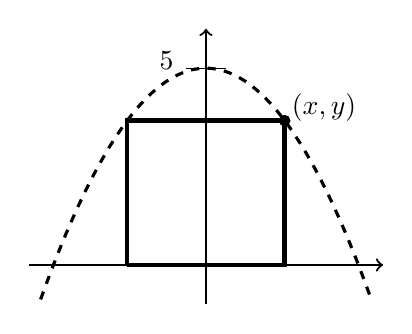
\begin{tikzpicture}[scale=.5]
\draw[thick, ->] (0,-1) -- (0,6);
\draw[thick, ->] (-4.5,0) -- (4.5,0);
\draw (-.5,5) -- (0.5,5);
\node at (-1,5.2){5};
\draw[ultra thick] (-2,0)--(2,0) -- (2, 3.666) -- (-2,3.666) -- (-2,0);
\node[draw, circle, fill=black,scale=0.4] at (2,3.666){};
\node at (3,4){$(x,y)$};
\draw[black, line width = 0.40mm, dashed]   plot[smooth,domain=-4.2:4.2] (\x, {5-0.333*\x*\x});
\end{tikzpicture}
\begin{subproblems}
\item Identify the objective function. That is, identify the quantity to be maximized or minimized.
\vspace{0.4in}
\item Write the objective function as a function of $x.$
\vspace{1in}
\item Answer the question and use Calculus to demonstrate that you answer is correct. (That is, you need to show that you have found a minimum or maximum.)
\vfill
Dimensions of the largest rectangle are: \quad \textbf{base}$=$ \underline{\hspace{1in}}\quad  \textbf{height}$=$ \underline{\hspace{1in}}
\end{subproblems}

\newpage
\problem{9} Evaluate the following limits. You must show your work to earn full credit. If you apply L'Hopital's Rule, you should indicate this.
\begin{subproblems}
\item $\displaystyle{\lim_{x\to 0} \frac{2e^x-2x-2}{3x^2}}$
\vfill
\item $\displaystyle{\lim_{x\to 0} \frac{2x^2-5x}{\cos(x)}}$
\vfill
\item $\displaystyle{\lim_{x\to 0^+} x \ln(x^4)}$
\vfill

\end{subproblems}

\problem{8} Evaluate the following indefinite integrals. You must show your work to earn full credit. If you apply L'Hopital's Rule, you should indicate this.
\begin{subproblems}
\item $\displaystyle{\int (x^{1/2}+\sin(x) + 5e^x) \: dx}$
\vfill
\item $\displaystyle{\int \left(\sec^2(x)+\frac{x+1}{x} \right) dx}$
\vfill

\end{subproblems}
\end{document}